\documentclass{article}
\usepackage{fancyhdr}
\usepackage{ctex}
\usepackage{listings}
\usepackage{graphicx}
\usepackage[a4paper, body={18cm,22cm}]{geometry}
\usepackage{amsmath,amssymb,amstext,wasysym,enumerate,graphicx}
\usepackage{float,abstract,booktabs,indentfirst,amsmath}
\usepackage{array}
\usepackage{booktabs}
\usepackage{multirow}
\usepackage{url}
\usepackage{diagbox}
\renewcommand\arraystretch{1.4}
\usepackage{indentfirst}
\setlength{\parindent}{2em}
\usepackage{enumitem}
\setmonofont{Consolas}
\usepackage{listings}
\usepackage{xcolor}
\usepackage{makecell}
\setCJKmonofont{黑体}
\lstset{
    % language = C,
    xleftmargin = 3em,xrightmargin = 3em, aboveskip = 1em,
	backgroundcolor = \color{white}, % 背景色
	basicstyle = \small\ttfamily, % 基本样式 + 小号字体
	rulesepcolor= \color{gray}, % 代码块边框颜色
	breaklines = true, % 代码过长则换行
	numbers = left, % 行号在左侧显示
	numberstyle = \small, % 行号字体
    numbersep = -14pt, 
    keywordstyle=\color{purple}\bfseries, % 关键字颜色
    commentstyle =\color{red!50!green!50!blue!60}, % 注释颜色
    stringstyle = \color{red}, % 字符串颜色
    morekeywords={ASSERT, int64_t, uint32_t},
	frame = shadowbox, % 用(带影子效果)方框框住代码块
	showspaces = false, % 不显示空格
	columns = fixed, % 字间距固定
} 
\lstset{
    sensitive=true,
    moreemph={ASSERT, NULL}, emphstyle=\color{red}\bfseries,
    moreemph=[2]{int64_t, uint32_t, tid_t, uint8_t, int16_t, uint16_t, int32_t, size_t}, emphstyle=[2]\color{purple}\bfseries,
    }
%--------------------页眉--------------------%
\pagestyle{fancy}
\fancyhead[L]{}
\fancyhead[R]{}
\fancyhead[C]{华东师范大学软件工程学院实验报告}
\fancyfoot[C]{-\thepage-}
\renewcommand{\headrulewidth}{1.5pt}
%--------------------标题--------------------%
\begin{document}
\begin{center}
  \LARGE{{\textbf{\heiti 华东师范大学软件工程学院实验报告}}}
  \begin{table}[H]
    \centering
    \begin{tabular}{p{2cm}p{4cm}<{\centering}p{1cm}p{2cm}p{4cm}<{\centering}}
      实验课程:    & 计算机网络 & \quad & 年\qquad 级: & 2022级         \\ \cline{2-2} \cline{5-5}
      实验编号:    & Lab 01     & \quad & 实验名称:    & Protocol Layer
      \\ \cline{2-2} \cline{5-5}
      姓\qquad 名: & 李鹏达     & \quad & 学\qquad 号: & 10225101460    \\ \cline{2-2} \cline{5-5}
    \end{tabular}
  \end{table}
\end{center}
\rule{\textwidth}{1pt}
%--------------------正文--------------------%
\section{实验目的}
\begin{enumerate}[noitemsep, label={{\arabic*})}]
  \item 学会通过Wireshark获取各协议层的数据包
  \item 掌握协议层数据包结构
  \item 分析协议开销
\end{enumerate}
\section{实验内容与实验步骤}
\subsection{实验内容}


\subsubsection{获取协议层的数据包}
使用\texttt{wget}命令发起\texttt{HTTP}请求,然后使用\texttt{Wireshark}抓包。

\subsubsection{绘制数据包结构}

分析\texttt{HTTP} \texttt{GET}协议包的内容,并绘制协议包,分别标出\texttt{Ethernet},\texttt{IP}和\texttt{TCP}协议的头部的位置、大小以及其负载的范围。

\subsubsection{分析协议开销}

根据实验结构,分析\texttt{HTTP}应用协议额外开销。
估计上面捕获的\texttt{HTTP}协议的额外开销。
假设\texttt{HTTP}数据(头部和消息)是有用的,而\texttt{TCP},\texttt{IP}和\texttt{Ethernet}头部认为是开销。对于下载的主要部分中的每一个包,我们需要分析\texttt{Ethernet},\texttt{IP}和\texttt{TCP}的开销,和有用的\texttt{HTTP}数据的开销。根据以上的定义来估计下载协议的开销,你认为这种开销是必要的吗?

\subsubsection{分析解复用键}

\textbf{解复用}指找到正确的上一层协议来处理到达的包。

观察下载的以太网和\texttt{IP}包头部信息,回答下面问题:

\begin{enumerate}[noitemsep]
  \item 以太网头部中哪一部分是解复用键并且告知它的下一个高层指的是\texttt{IP},在这一包内哪一个值可以表示\texttt{IP}?
  \item \texttt{IP}头部中哪一部分是解复用键并且告知它的下一一个高层指的是TCP,在这一包内哪一个值可以表示\texttt{TCP}?
\end{enumerate}

\subsubsection{问题讨论}

\begin{enumerate}[noitemsep]
  \item Look at a short TCP packet that carries no higher-layer data. To what entity is this packet destined? After all, if it carries no higher-layer data then it does not seem very useful to a higher layer protocol such as HTTP!
  \item In a classic layered model, one message from a higher layer has a header appended by the lower layer and becomes one new message. But this is not always the case. Above, we saw a trace in which the web response (one HTTP message comprised of an HTTP header and an HTTP payload) was converted into multiple lower layer messages (being multiple TCP packets).  Imagine that you have drawn the packet structure (as in step 2) for the first and last TCP packet carrying the web response.  How will the drawings differ?
  \item In the classic layered model described above, lower layers append headers to the messages passed down from higher layers. How will this model change if a lower layer adds encryption?
  \item In the classic layered model described above, lower layers append headers to the messages passed down from higher layers. How will this model change if a lower layer adds compression?
\end{enumerate}


\subsection{实验步骤}

\begin{enumerate}[noitemsep, label={{\arabic*})}]
  \item 安装实验所需软件(为方便安装,我们使用\texttt{Windows}下的包管理器\texttt{winget})
        \begin{lstlisting}[language=bash]
    PS> winget install wget
    PS> winget install wireshark
    \end{lstlisting}
  \item 打开\texttt{Wireshark},在菜单栏的 \texttt{捕获 -> 选项} 中进行设置,选择已连接的网络,设置捕获过滤器为\texttt{tcp port 80},将混杂模式设为关闭,勾选 \texttt{enable network  name resolution},然后开始捕获。
  \item 使用 \texttt{wget} 命令发起 \texttt{HTTP} 请求
        \begin{lstlisting}[language=bash]
    PS> wget http://www.baidu.com
    \end{lstlisting}
  \item 在 \texttt{Wireshark} 中停止捕获。
  \item 分析\texttt{HTTP} \texttt{GET}协议包的内容,并绘制协议包。
  \item 分析协议开销
  \item 分析解复用键
  \item 问题讨论
\end{enumerate}

\section{实验环境}


\begin{itemize}[noitemsep]
  \item 操作系统:\texttt{Windows 11 家庭中文版 23H2 22631.2715}
  \item 网络适配器:\texttt{Killer(R) Wi-Fi 6 AX1650i 160MHz Wireless Network \\ Adapter(201NGW)}
  \item \texttt{Wireshark}:\texttt{Version 4.2.0 (v4.2.0-0-g54eedfc63953)}
  \item \texttt{wget}:\texttt{GNU Wget 1.21.4 built on mingw32}
\end{itemize}


\section{实验过程与分析}

\subsection{获取协议层的数据包}

首先,我们打开\texttt{Wireshark},在菜单栏的 \texttt{捕获 -> 选项} 中进行设置,选择已连接的网络,设置捕获过滤器为\texttt{tcp port 80},将混杂模式设为关闭,勾选 \texttt{enable network  name resolution},然后开始捕获。

\begin{figure}[H]
  \centering
  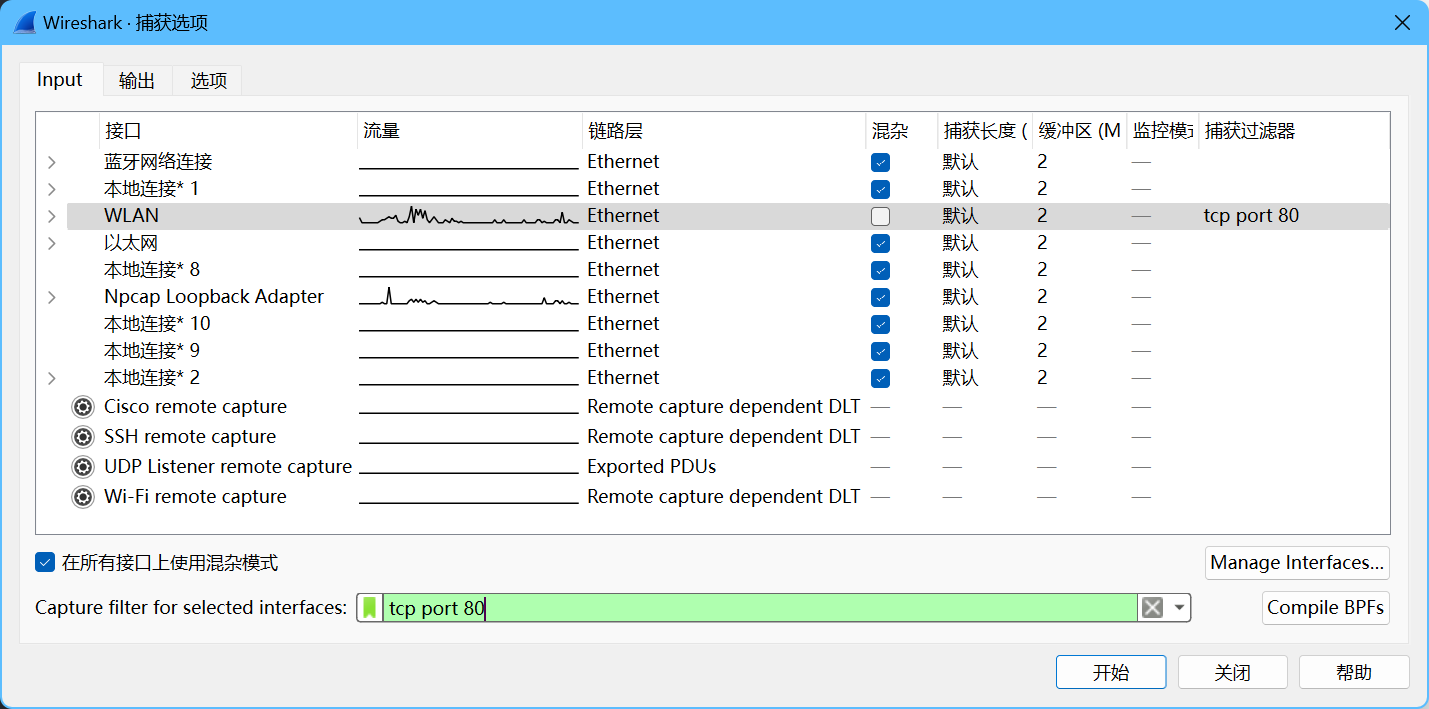
\includegraphics[width=15cm]{images/01.png}
  \caption{开始捕获}
\end{figure}

然后,我们使用 \texttt{wget} 命令对\texttt{http://www.baidu.com}发起 \texttt{HTTP} 请求

\begin{figure}[H]
  \centering
  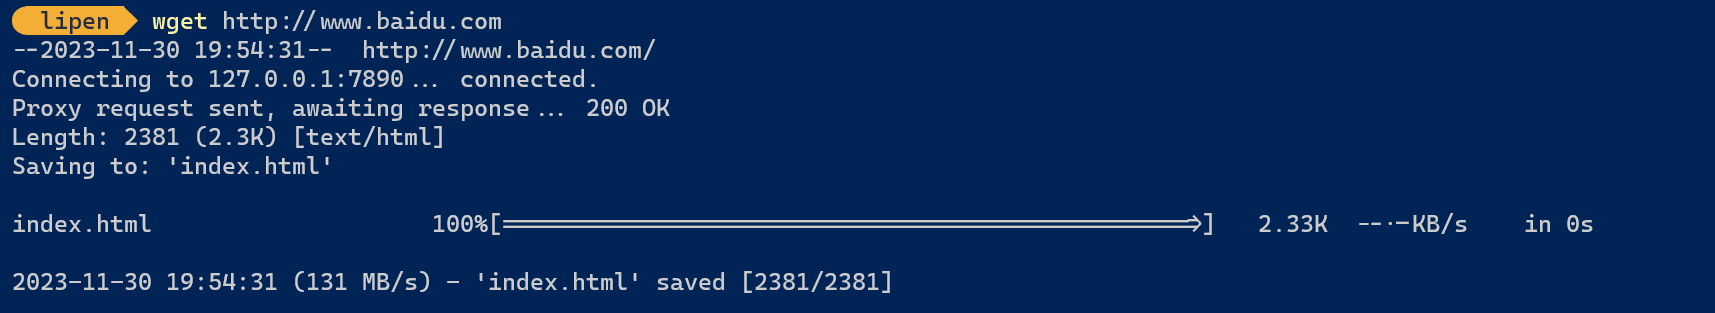
\includegraphics[width=15cm]{images/02.png}
  \caption{使用 \texttt{wget} 命令发起 \texttt{HTTP} 请求}
\end{figure}

最后,我们在 \texttt{Wireshark} 中停止捕获,得到如下结果:

\begin{figure}[H]
  \centering
  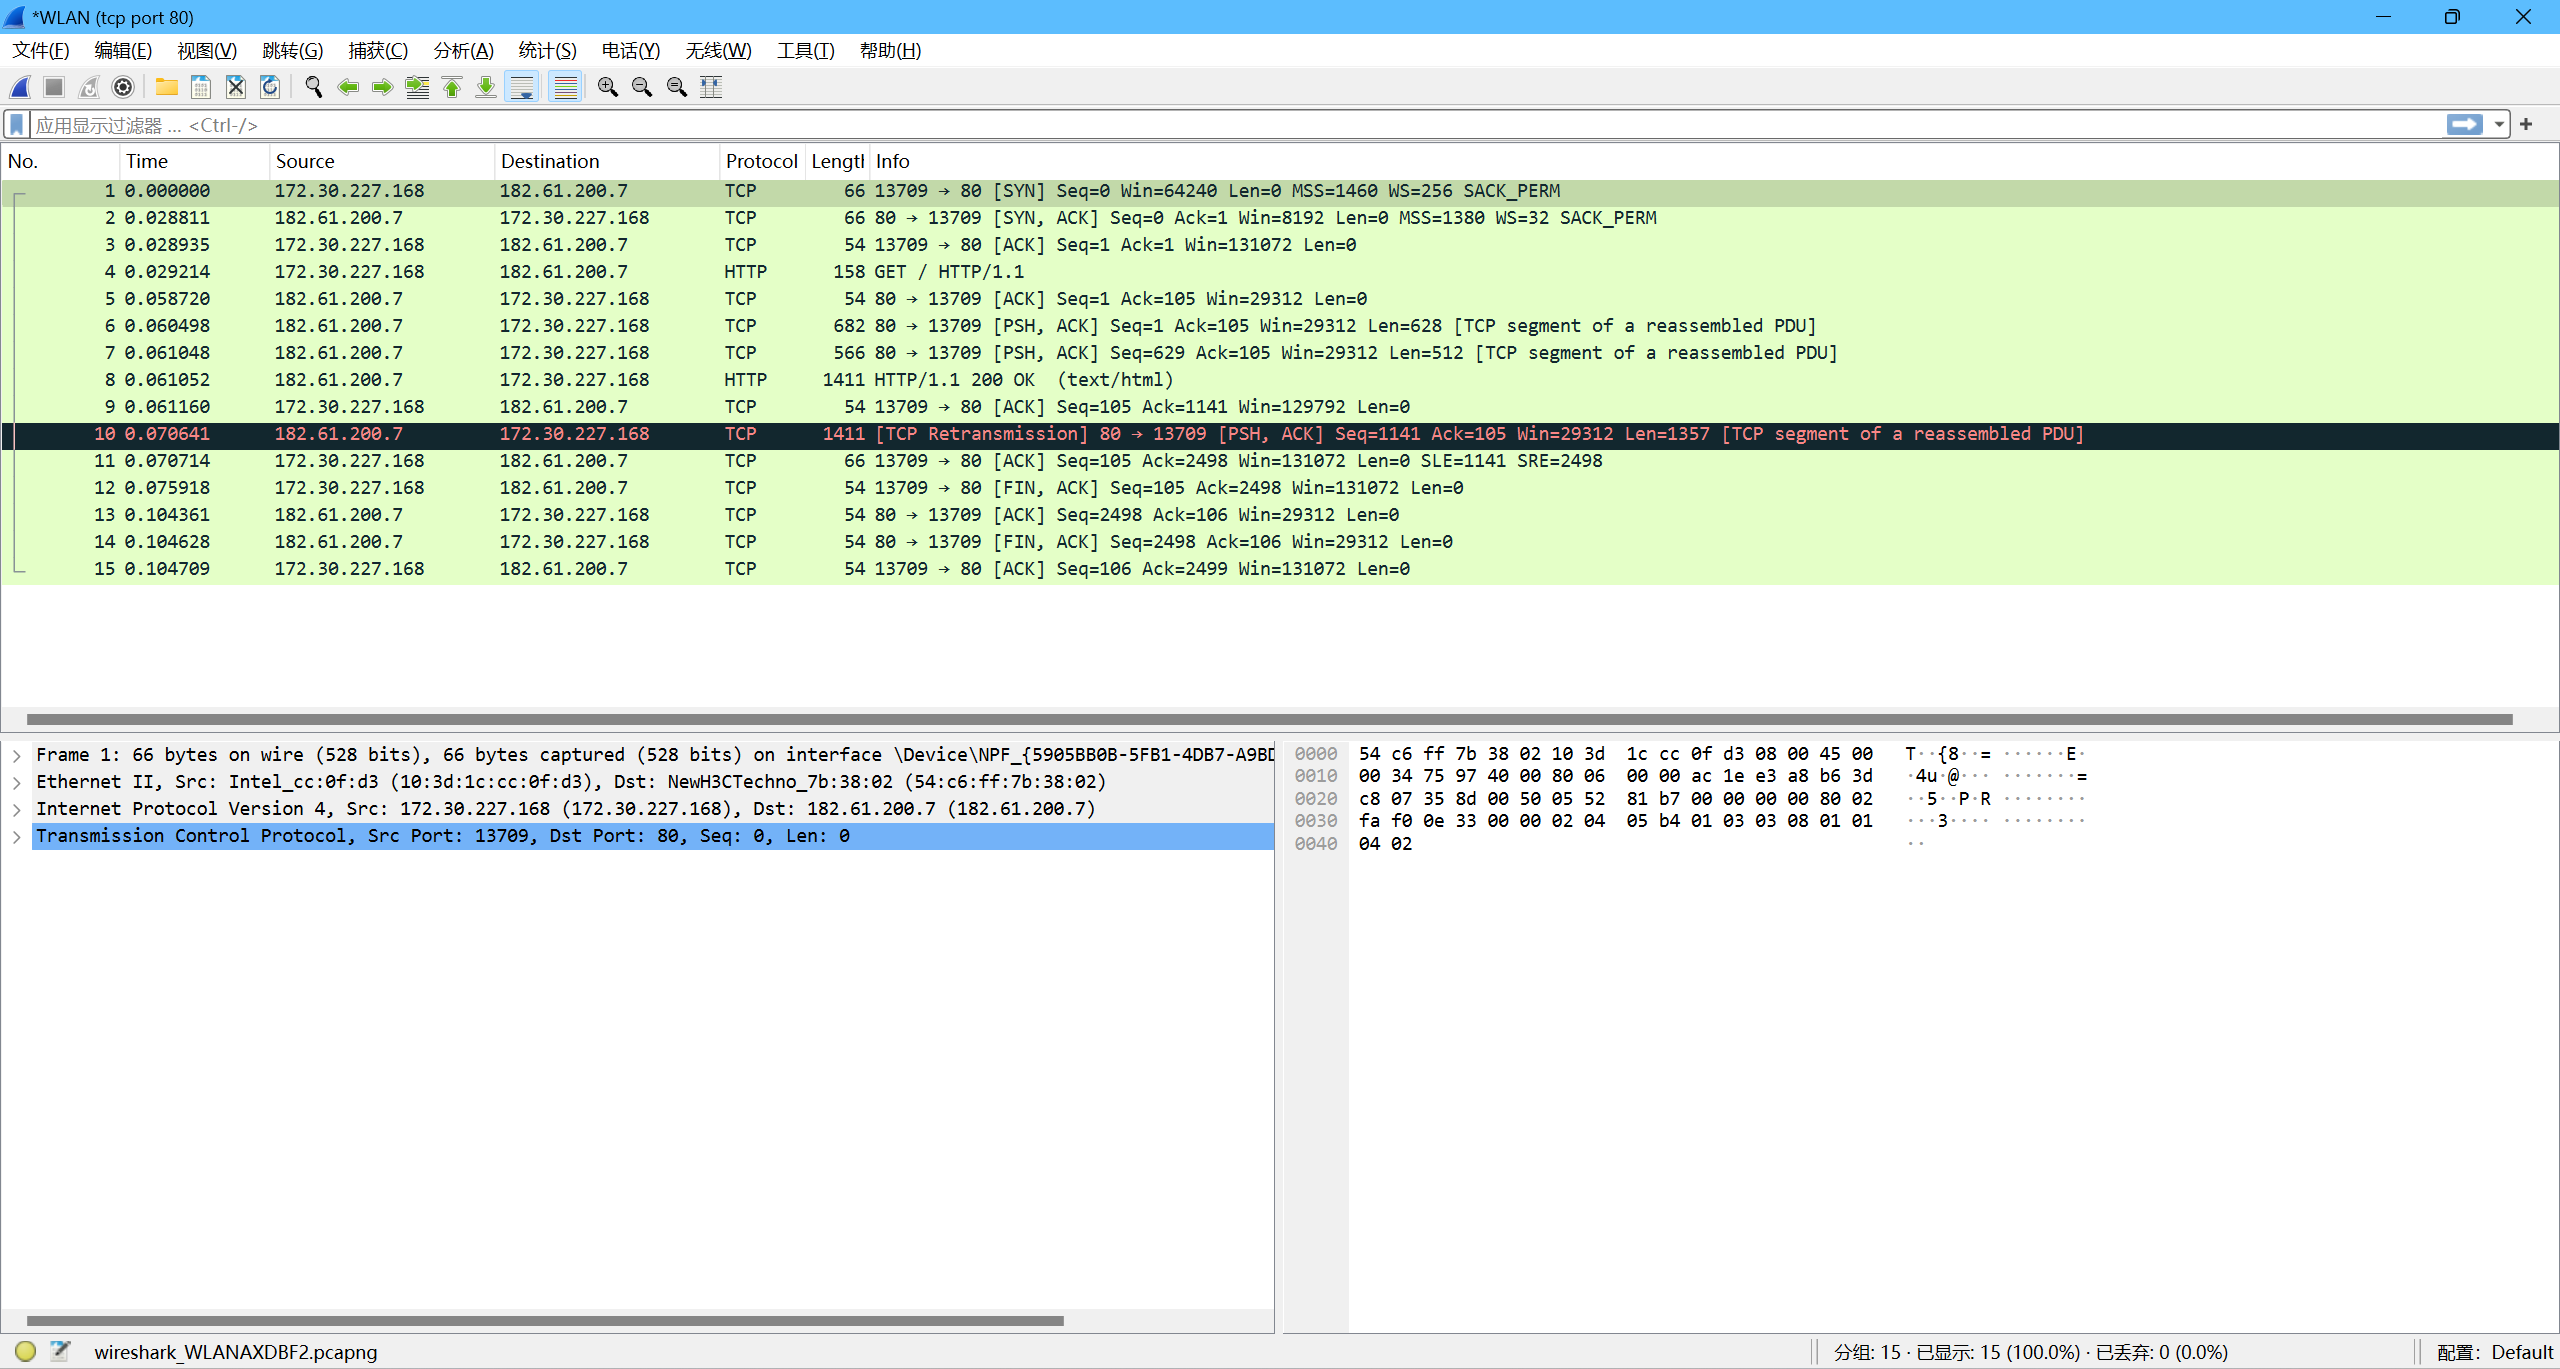
\includegraphics[width=15cm]{images/03.png}
  \caption{捕获结果}
\end{figure}

\subsection{绘制数据包结构}

接下来,我们分析数据包的结构。在\texttt{Wireshark}中,我们选择\texttt{HTTP} \texttt{GET}协议包,可以看到其内容,如下图所示:

\begin{figure}[H]
  \centering
  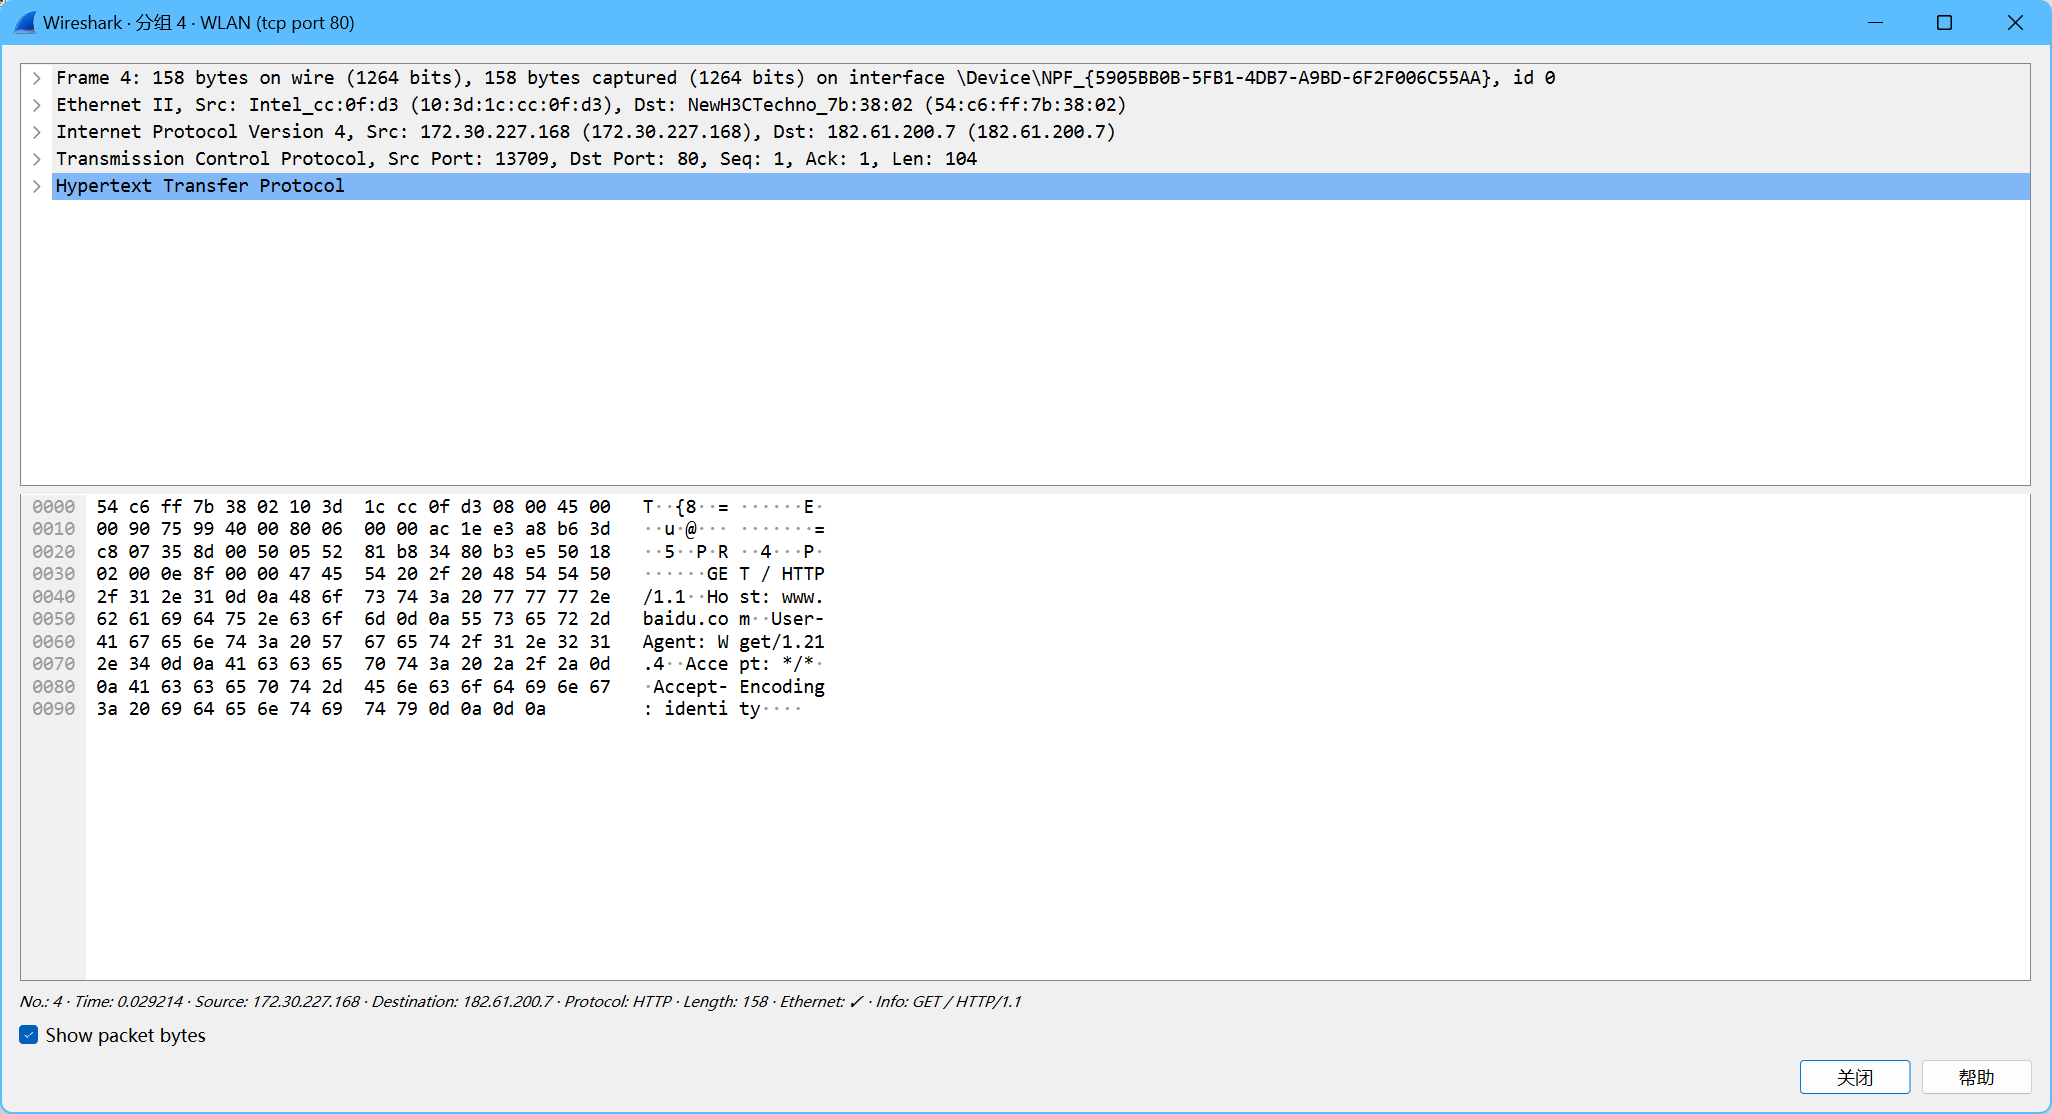
\includegraphics[width=15cm]{images/04.png}
  \caption{\texttt{HTTP} \texttt{GET}协议包}
\end{figure}

其中,第一个块是\texttt{Frame},这不是一个协议,而是一个记录,描述有关数据包的整体信息,包括捕获时间和长度等。我们可以看到,整个数据包的长度是\texttt{158}字节。
第二个块是\texttt{Ethernet II},这是以太网协议,可以看到这个标头的长度是\texttt{14}字节。
第三个块是\texttt{Internet Protocol Version 4},这是\texttt{IP}协议,可以看到这个标头的长度是\texttt{20}字节。
第四个块是\texttt{Transmission Control Protocol},这是\texttt{TCP}协议,可以看到这个标头的长度是\texttt{20}字节。
第五个块是\texttt{Hypertext Transfer Protocol},这是\texttt{HTTP}协议,可以看到这个标头的长度是\texttt{104}字节。

\begin{figure}[H]
  \centering
  \begin{minipage}[b]{0.45\textwidth}
    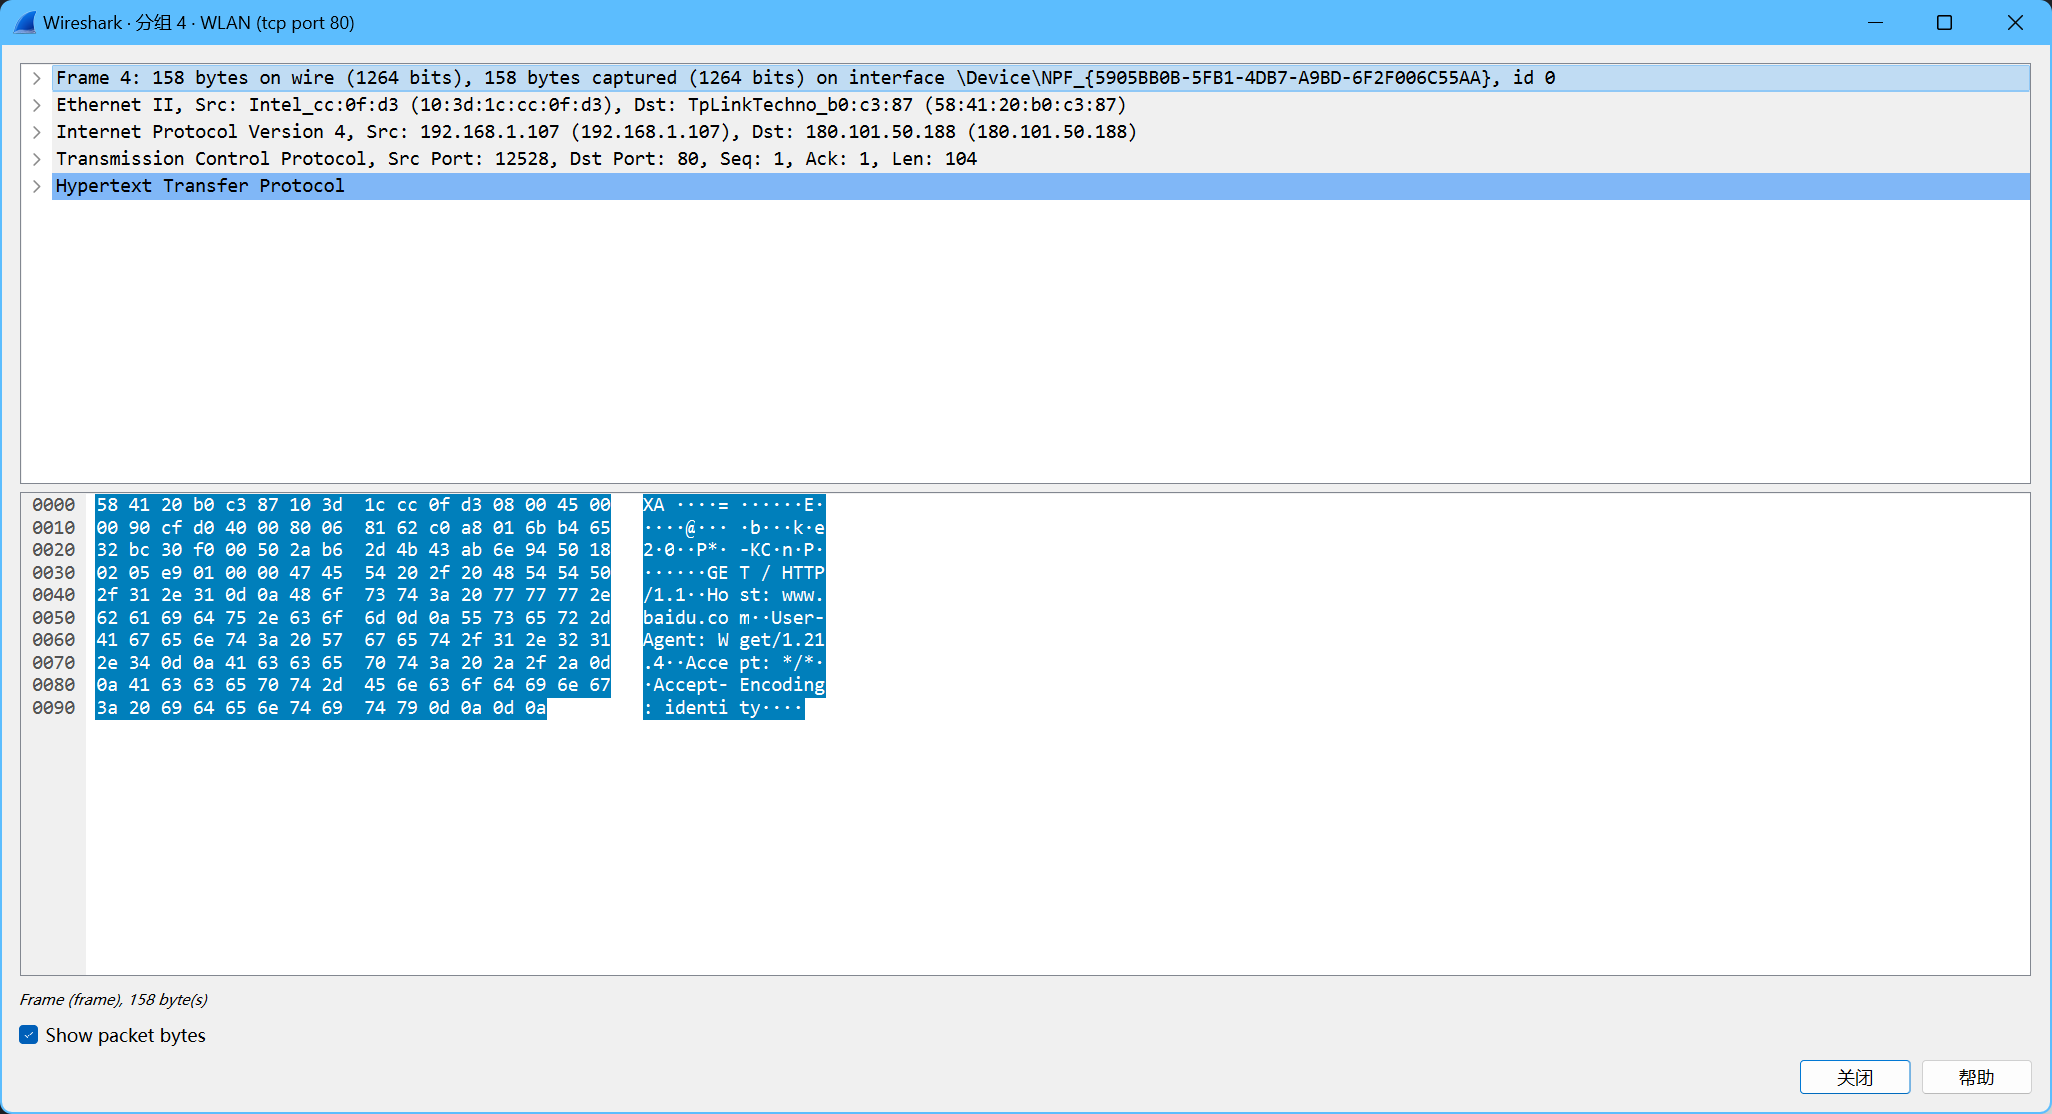
\includegraphics[width=\textwidth]{images/05.png}
    \caption{数据包的整体信息}
  \end{minipage}
  \hfill
  \begin{minipage}[b]{0.45\textwidth}
    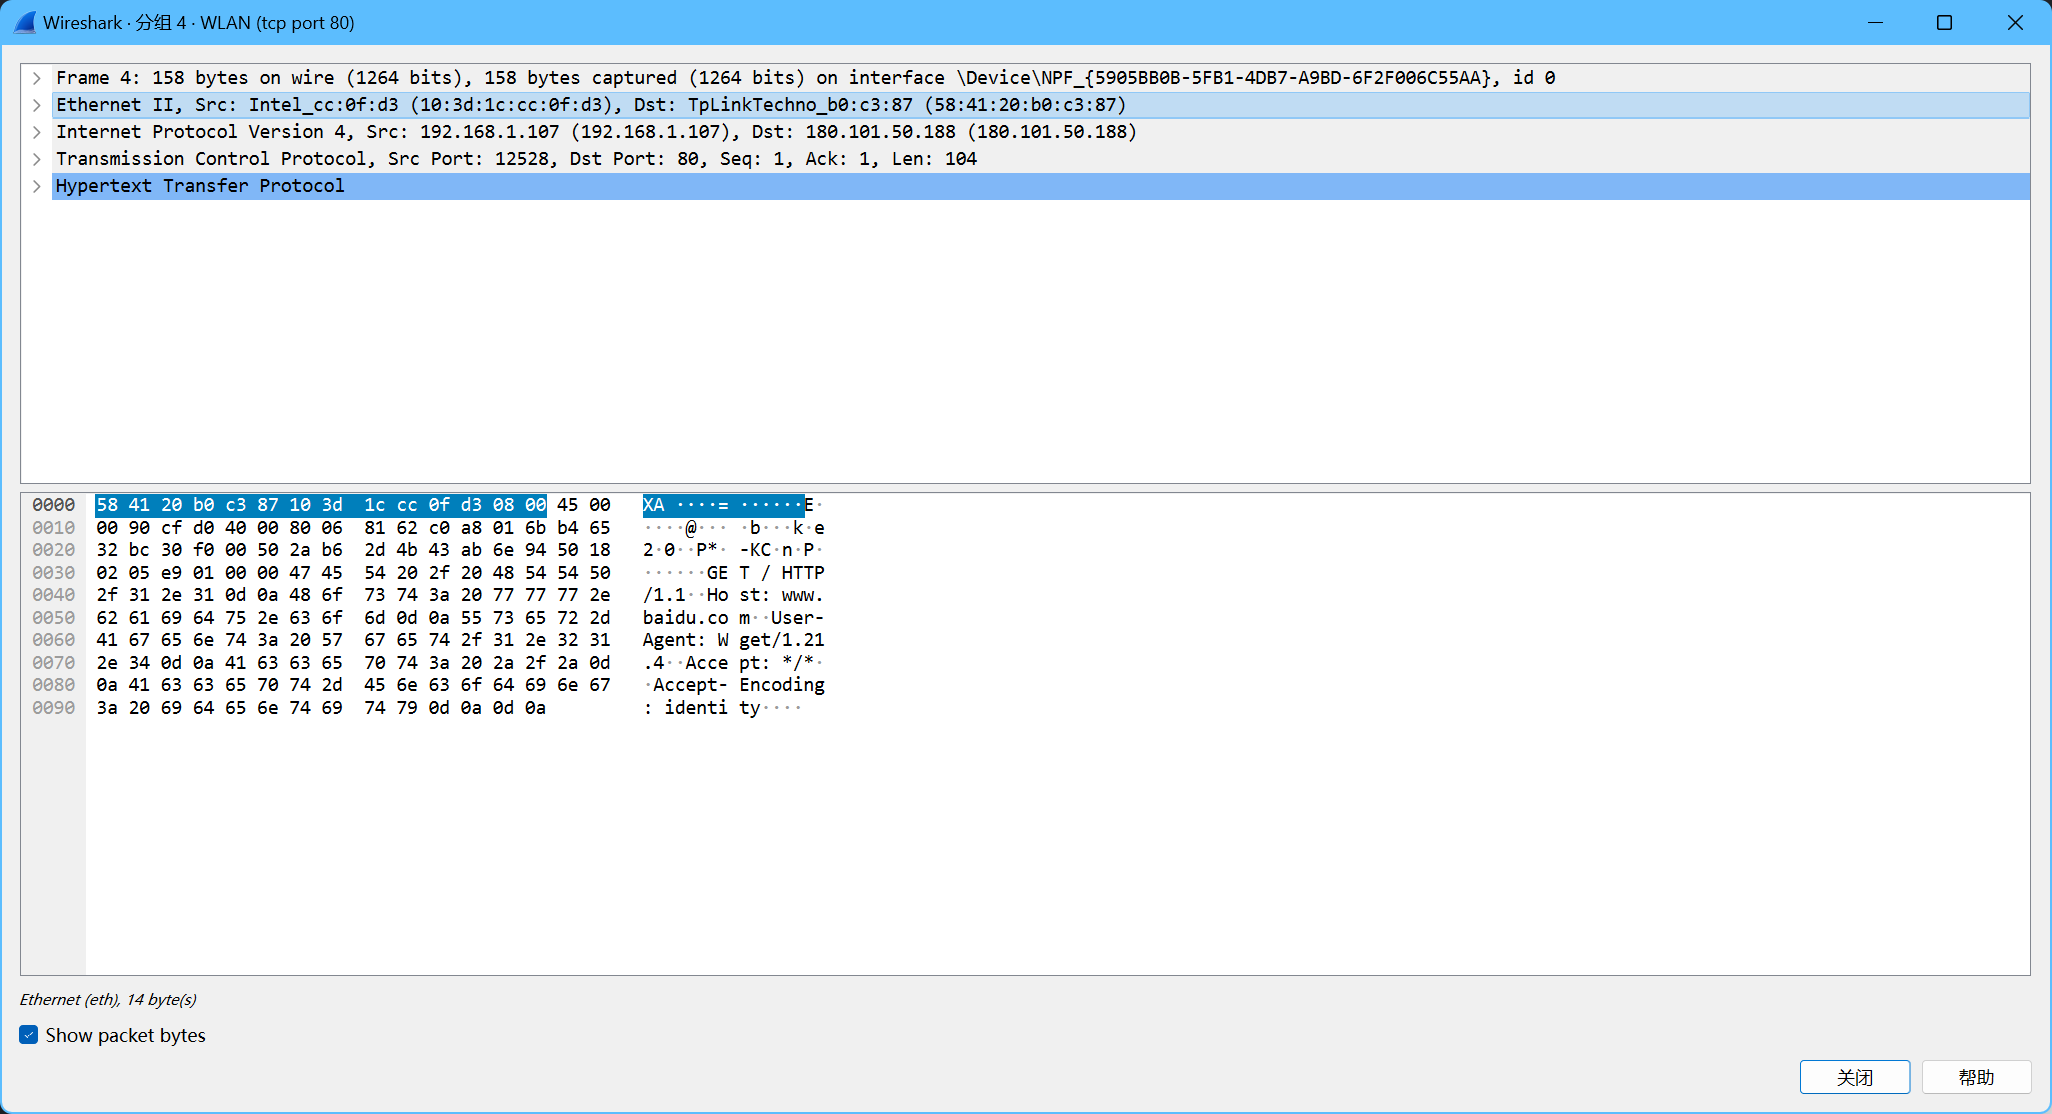
\includegraphics[width=\textwidth]{images/06.png}
    \caption{\texttt{以太网}协议包}
  \end{minipage}
\end{figure}

\begin{figure}[H]
  \centering
  \begin{minipage}[b]{0.45\textwidth}
    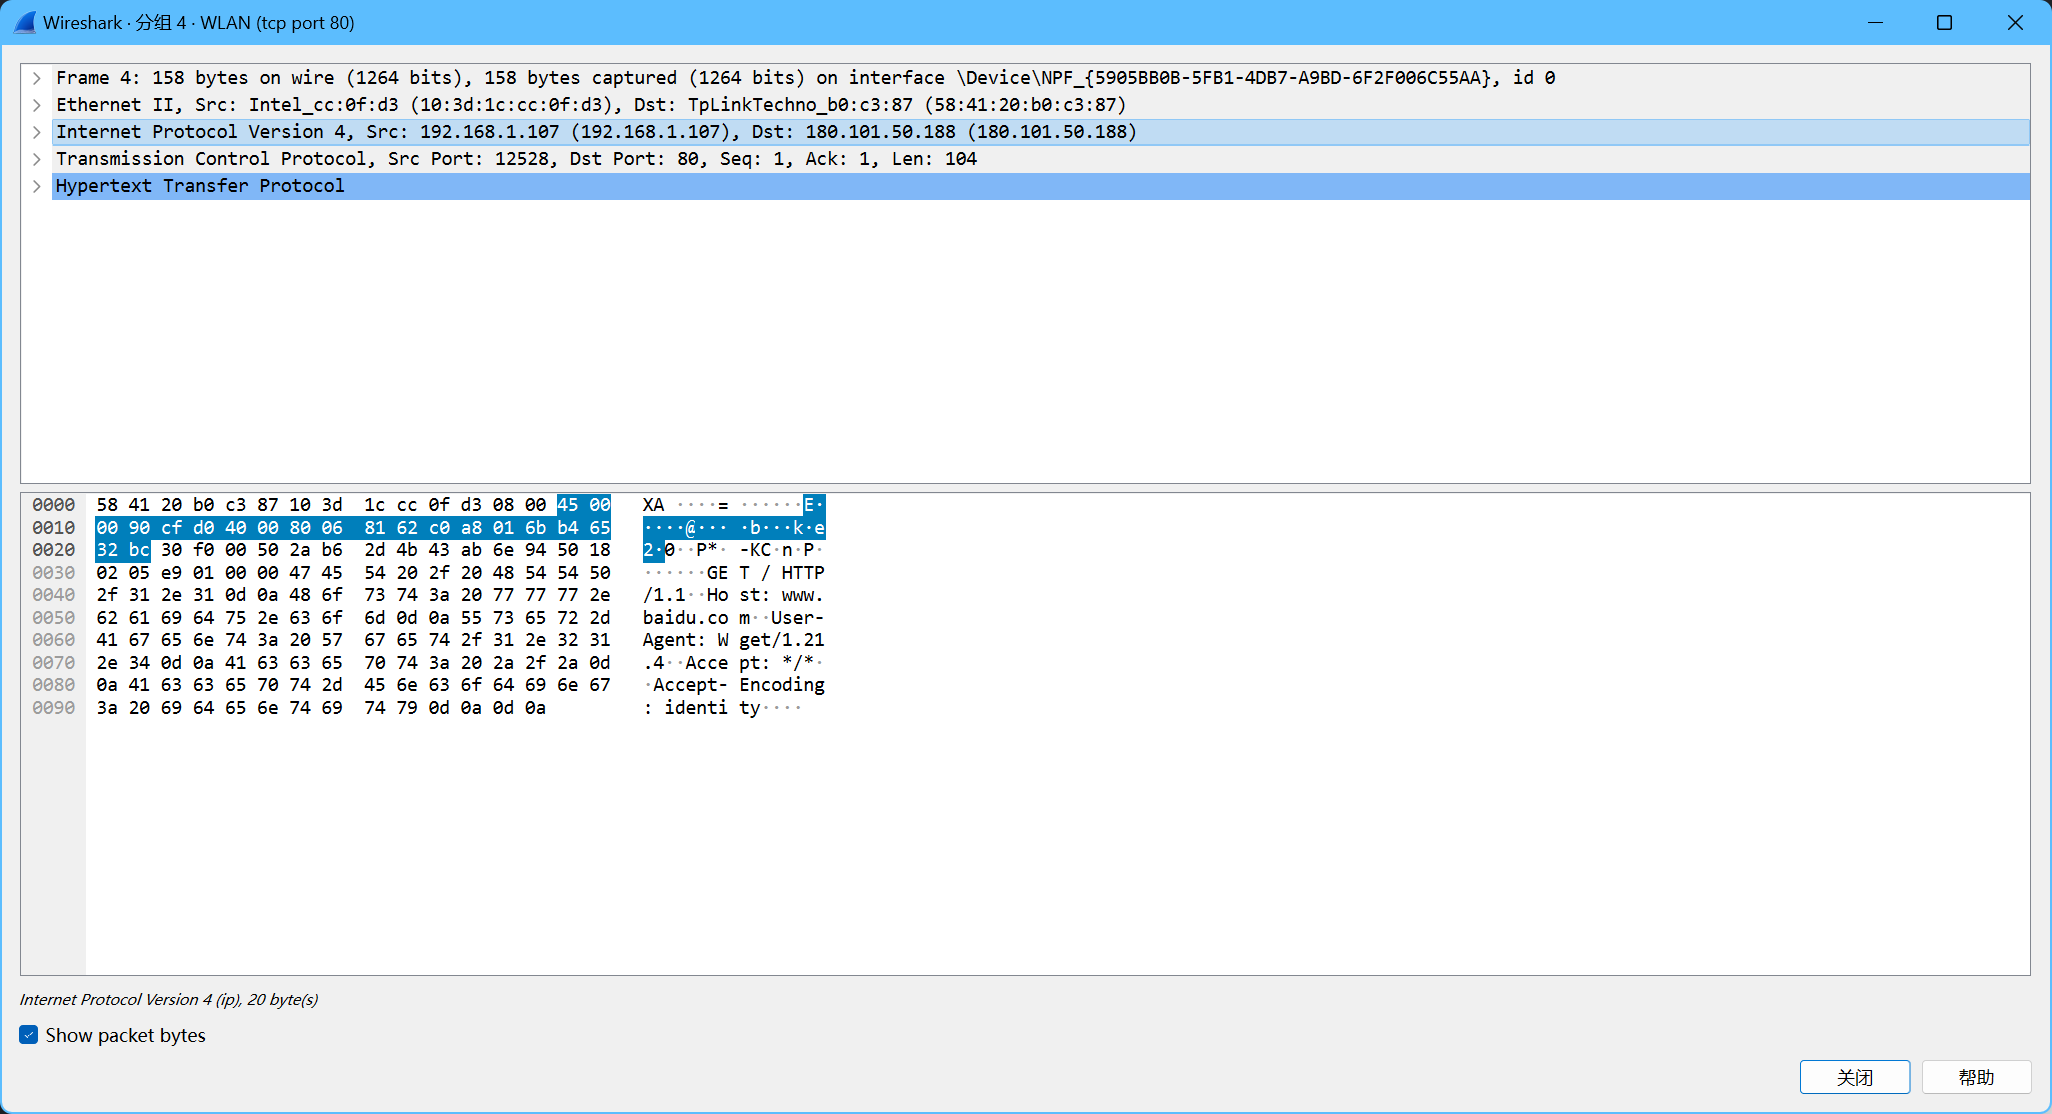
\includegraphics[width=\textwidth]{images/07.png}
    \caption{\texttt{IP}协议包}
  \end{minipage}
  \hfill
  \begin{minipage}[b]{0.45\textwidth}
    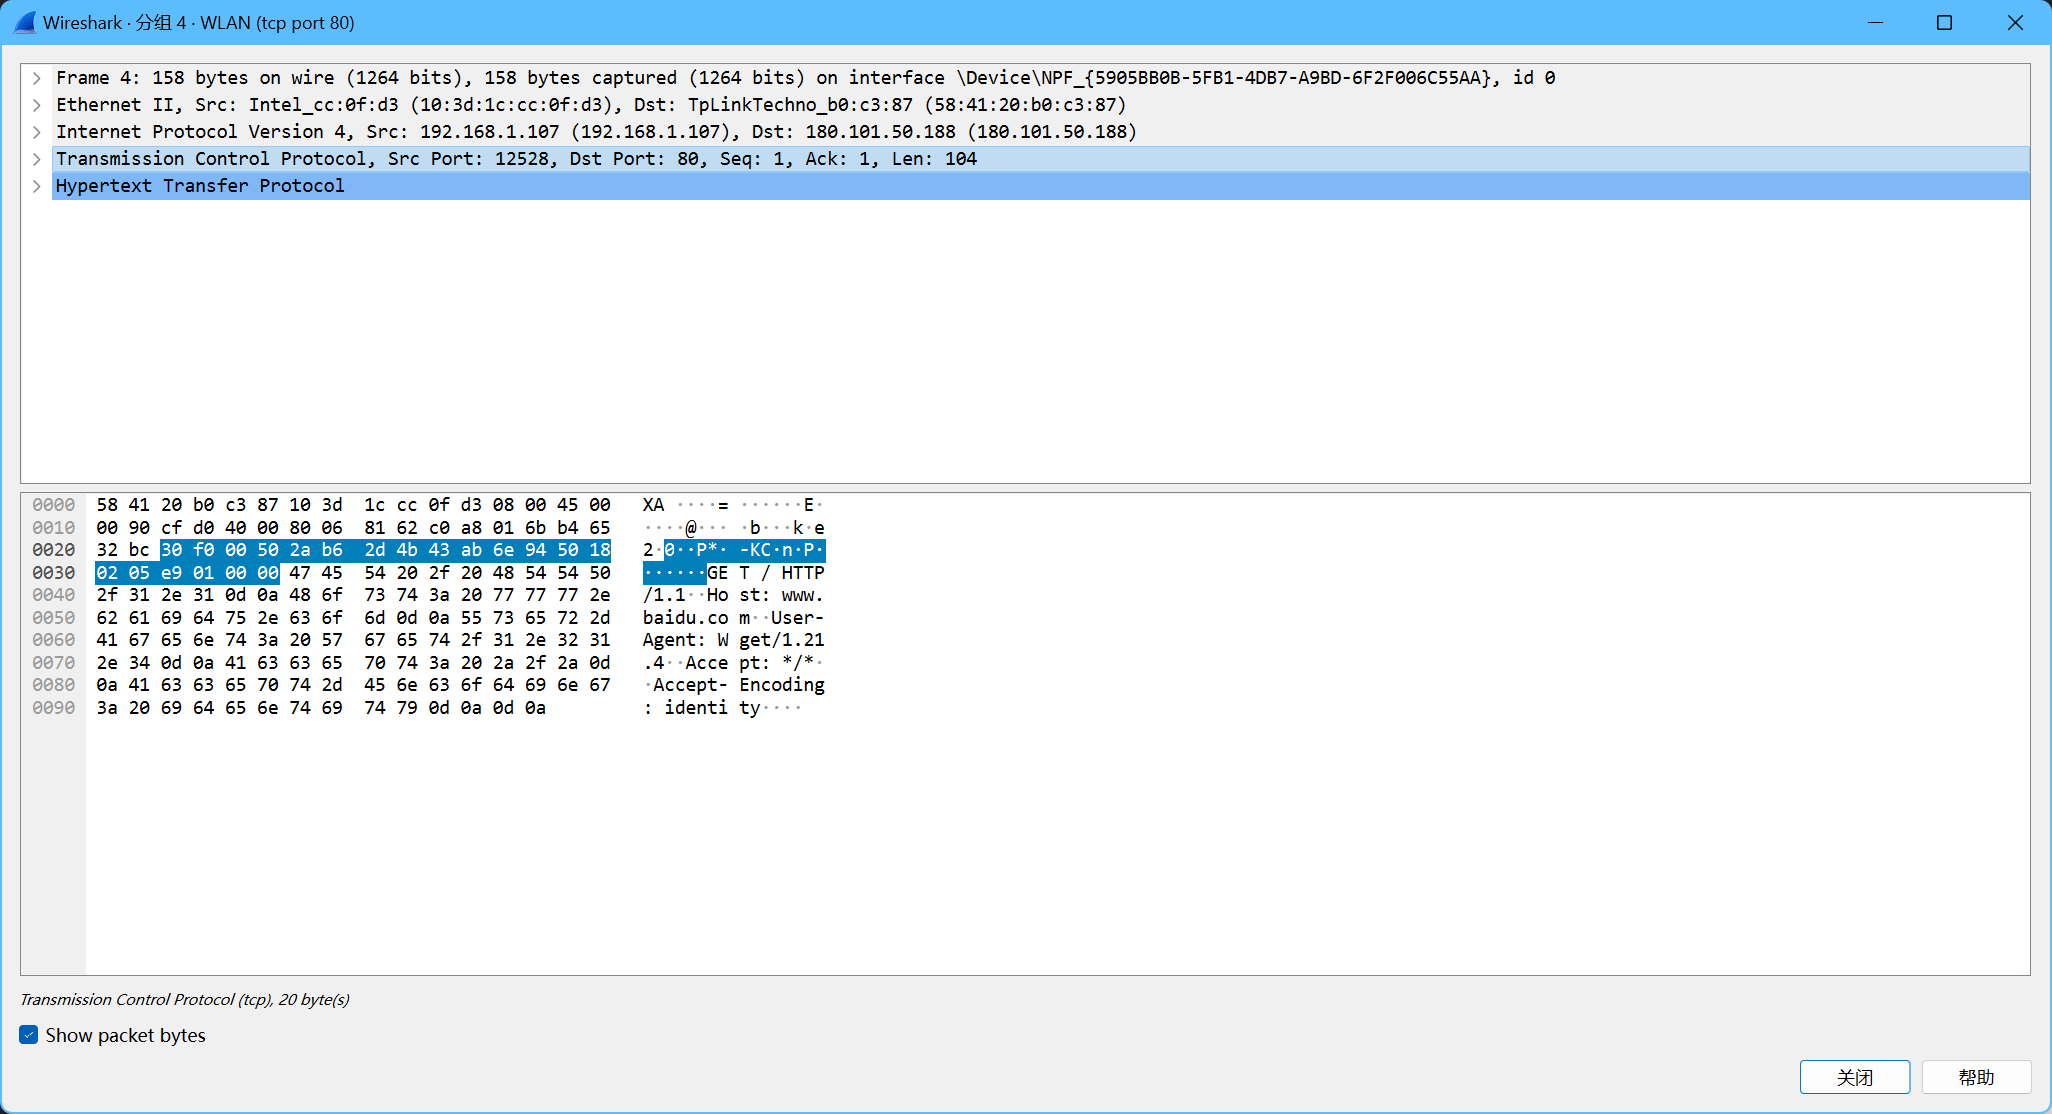
\includegraphics[width=\textwidth]{images/08.png}
    \caption{\texttt{TCP}协议包}
  \end{minipage}
\end{figure}

\begin{figure}[H]
  \centering
  \begin{minipage}[b]{0.45\textwidth}
    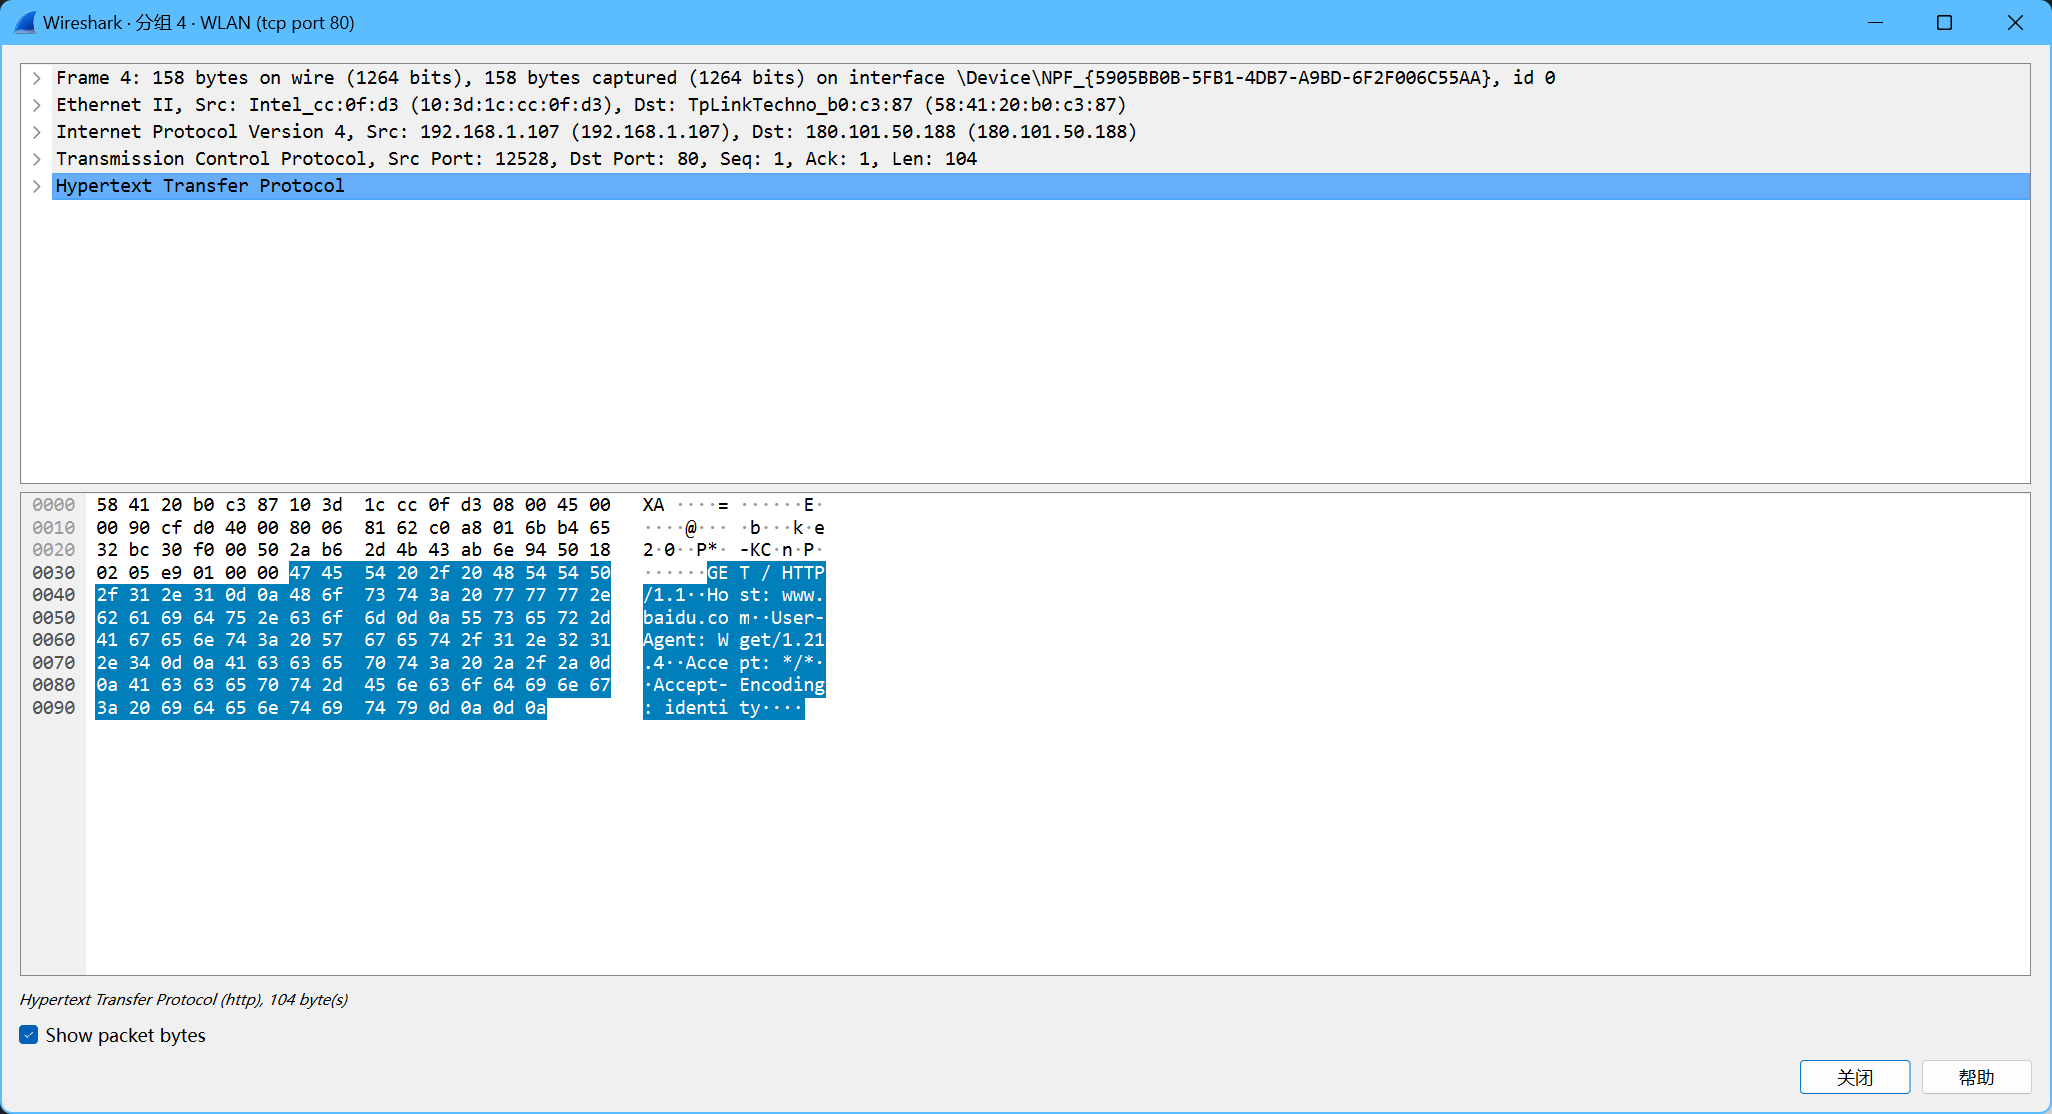
\includegraphics[width=\textwidth]{images/09.png}
    \caption{\texttt{HTTP}协议包}
  \end{minipage}
\end{figure}

协议包的结构如下图所示:

\begin{figure}[H]
  \centering
  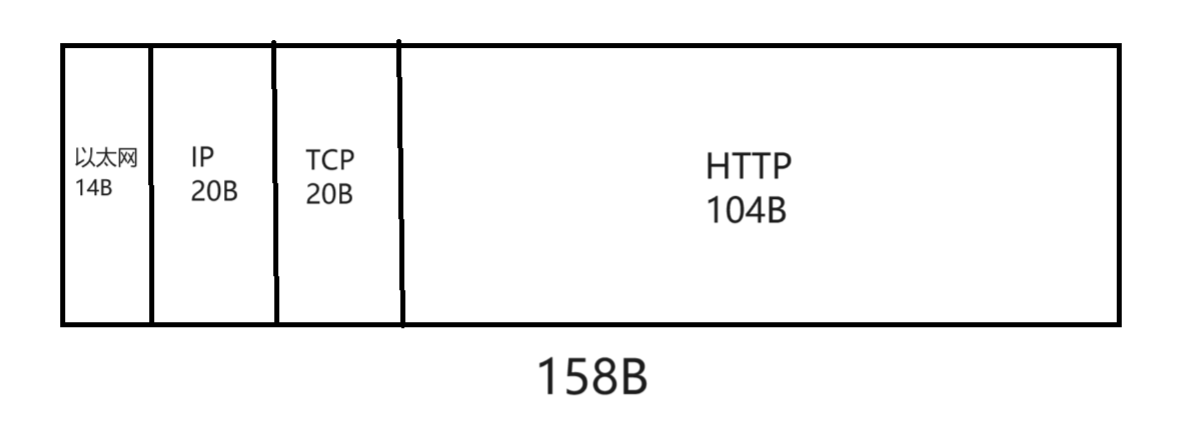
\includegraphics[width=15cm]{images/10.png}
  \caption{协议包的结构}
\end{figure}

\subsection{分析协议开销}

\texttt{以太网} 的开销为

$$
  \frac{14}{158}=8.86\%
$$

\texttt{IP} 的开销为

$$
  \frac{20}{158}=12.66\%
$$

\texttt{TCP} 的开销为

$$
  \frac{20}{158}=12.66\%
$$

整个捕获过程(从\texttt{SYN ACK}开始,
到\texttt{HTTP}后的第一个\texttt{TCP}数据包结束)的开销为

$$
  \frac{14+20+20+ 66 + 54 \times 2}{158 + 66 + 54 \times 2}= 68.7\%
$$

有用的\texttt{HTTP}数据的开销为

$$
  \frac{104}{158 + 66 + 54 \times 2}= 31.3\%
$$

\begin{figure}[H]
  \centering
  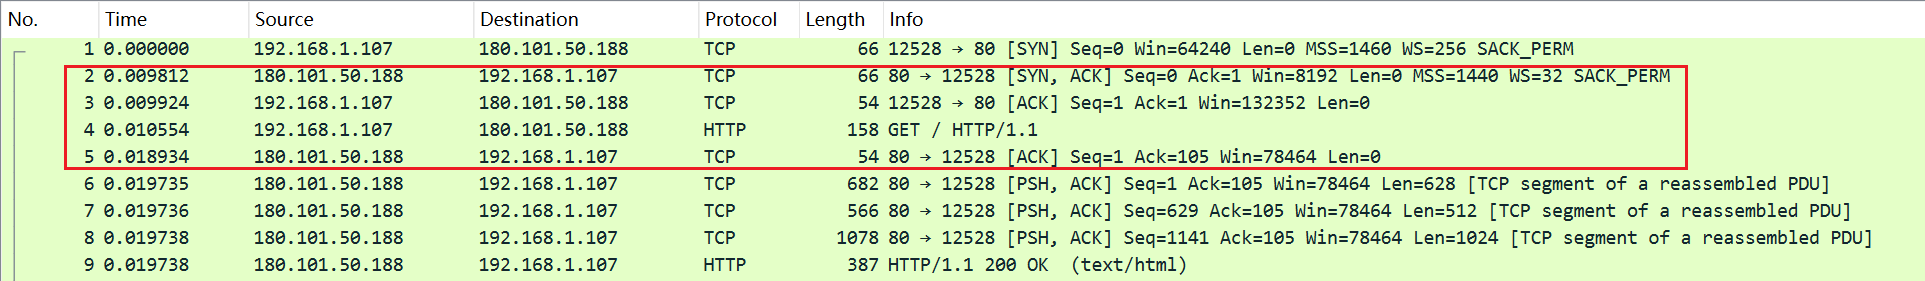
\includegraphics[width=15cm]{images/11.png}
  \caption{整个捕获过程}
\end{figure}

\subsection{分析解复用键}

\begin{enumerate}[noitemsep]
  \item 以太网头部中哪一部分是解复用键并且告知它的下一个高层指的是\texttt{IP},在这一包内哪一个值可以表示\texttt{IP}?

        \texttt{以太网}头部中的\texttt{type}字段是解复用键,它的值为\texttt{0x0800},表示\texttt{IP}协议。

  \item \texttt{IP}头部中哪一部分是解复用键并且告知它的下一一个高层指的是TCP,在这一包内哪一个值可以表示\texttt{TCP}?

        \texttt{IP}头部中的\texttt{protocol}字段是解复用键,它的值为\texttt{0x06},表示\texttt{TCP}协议。
\end{enumerate}

\begin{figure}[H]
  \centering
  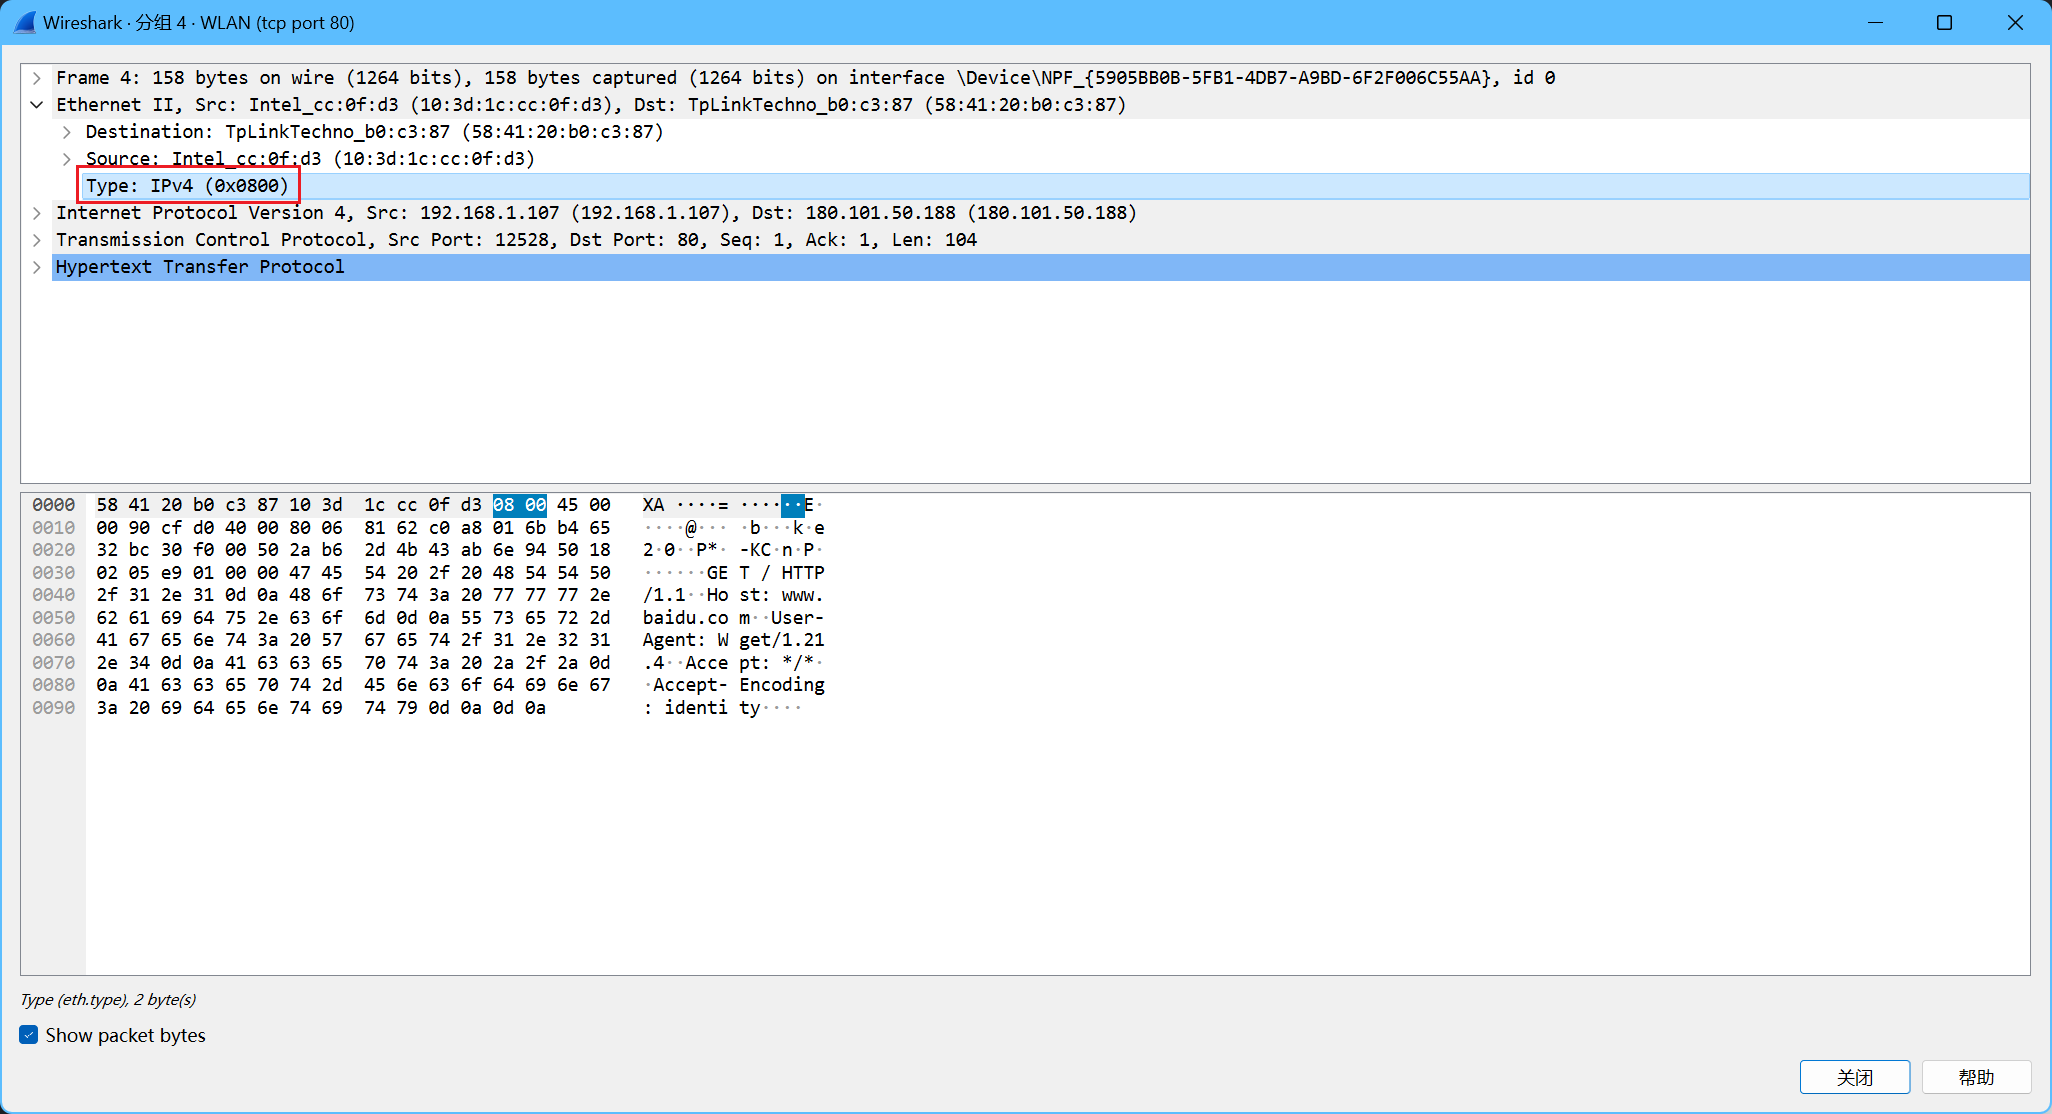
\includegraphics[width=13cm]{images/12.png}
  \caption{\texttt{以太网}头部}
\end{figure}

\begin{figure}[H]
  \centering
  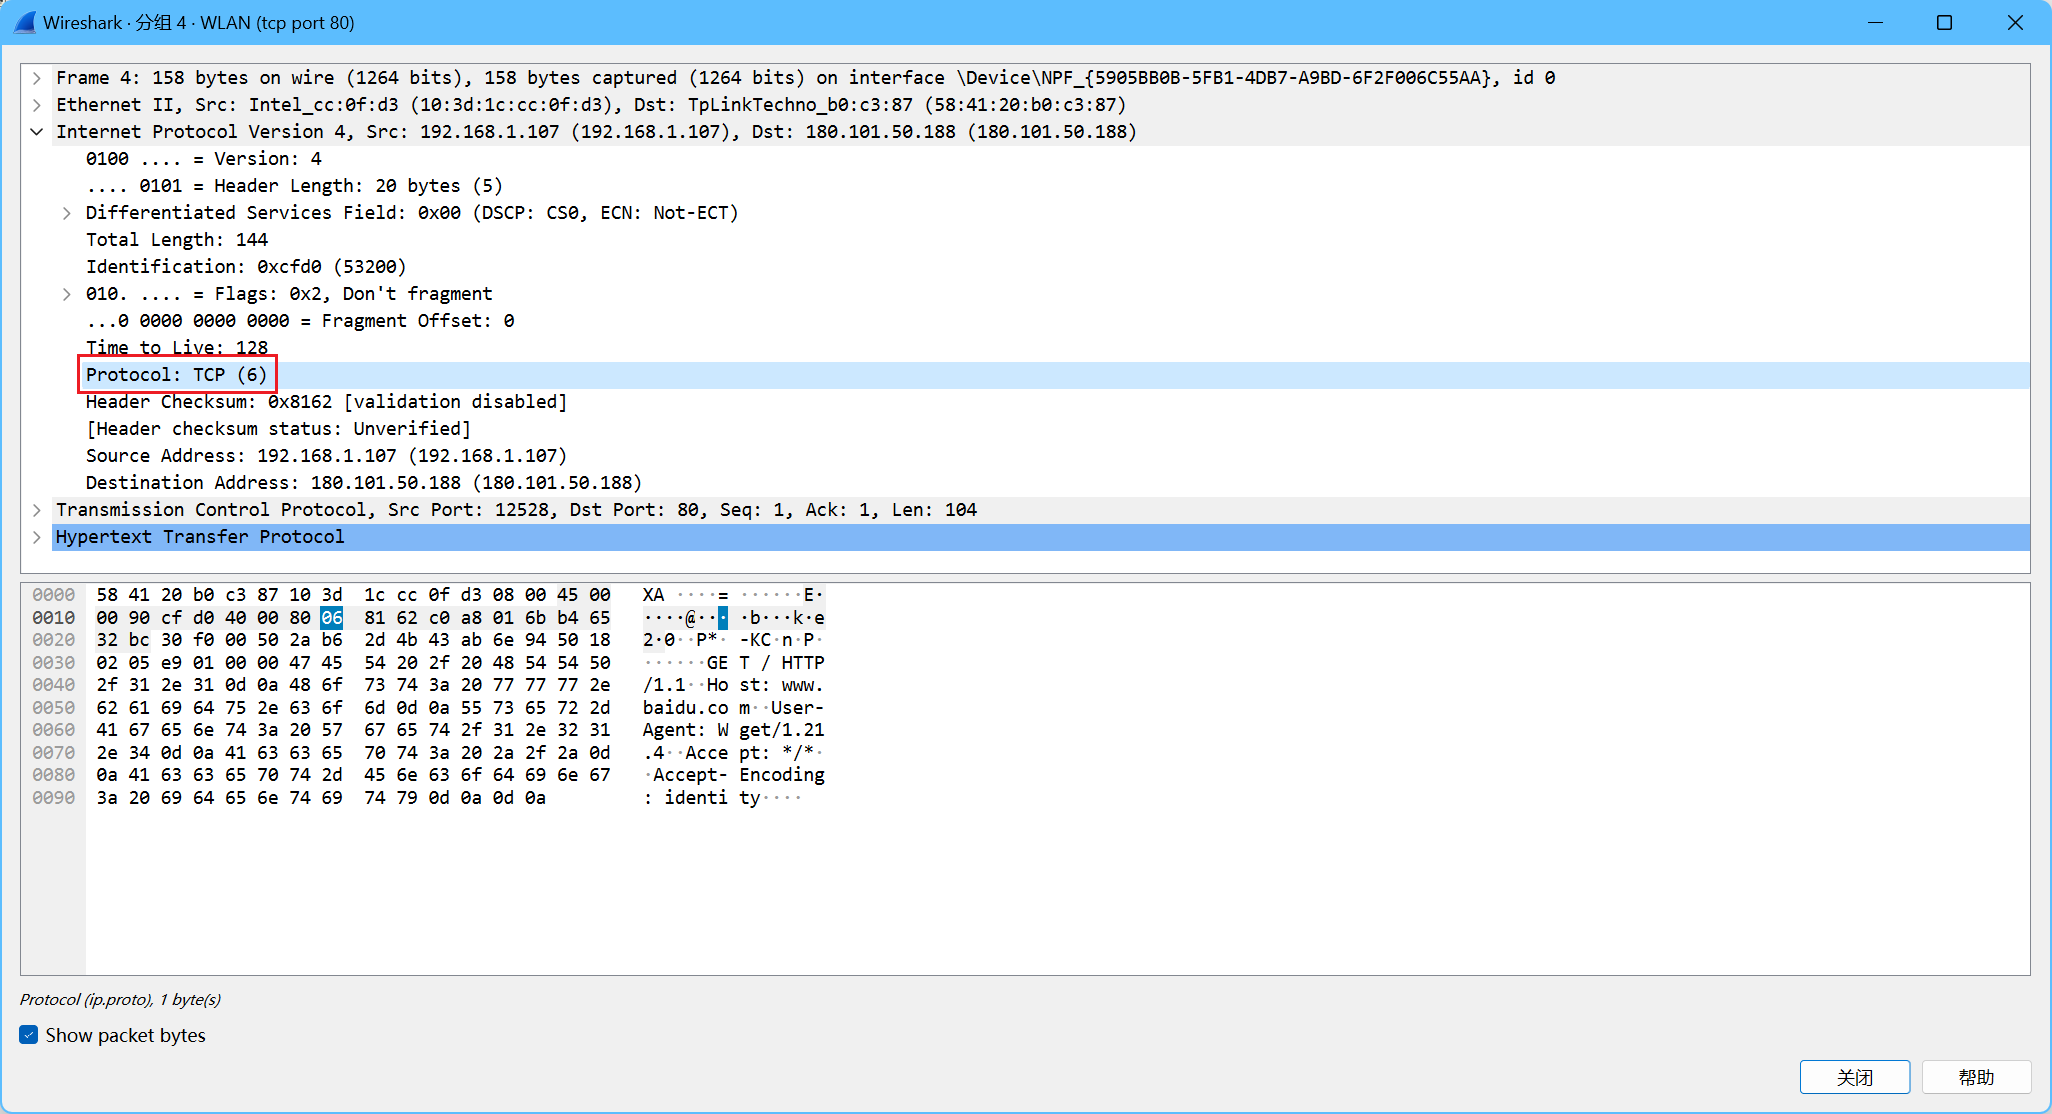
\includegraphics[width=13cm]{images/13.png}
  \caption{\texttt{IP}头部}
\end{figure}

\subsection{问题讨论}


\begin{enumerate}[noitemsep]
  \item Look at a short TCP packet that carries no higher-layer data. To what entity is this packet destined? After all, if it carries no higher-layer data then it does not seem very useful to a higher layer protocol such as HTTP!

        这个包的目的地是我们要访问的网站或者我们自己,通常是确认和控制信息类报文,用于建立\texttt{TCP}连接,对\texttt{HTTP}协议是有用的。这是\texttt{TCP}三次握手的一部分,用于建立\texttt{TCP}连接。

  \item In a classic layered model, one message from a higher layer has a header appended by the lower layer and becomes one new message. But this is not always the case. Above, we saw a trace in which the web response (one HTTP message comprised of an HTTP header and an HTTP payload) was converted into multiple lower layer messages (being multiple TCP packets).  Imagine that you have drawn the packet structure (as in step 2) for the first and last TCP packet carrying the web response.  How will the drawings differ?

        第一个\texttt{TCP}数据包的负载是\texttt{HTTP}协议的头部,而其余\texttt{TCP}数据包的负载是\texttt{HTTP}的有效载荷。


  \item In the classic layered model described above, lower layers append headers to the messages passed down from higher layers. How will this model change if a lower layer adds encryption?

        双方需要协商加密算法,然后在传输数据时,接收方需要解密数据,否则无法解析数据包。

  \item In the classic layered model described above, lower layers append headers to the messages passed down from higher layers. How will this model change if a lower layer adds compression?

        发送方可以将解压缩方法附在头部,接收方在接收到数据包后,可以解压缩数据包,然后解析数据包。

\end{enumerate}

\section{实验结果总结}

通过本次实验,我学会了通过\texttt{Wireshark}获取各协议层的数据包,掌握了协议层数据包结构,分析了协议开销,分析了解复用键。对计算机网络中的协议层有了更深的理解。

\section{附录}

无

\end{document}